\documentclass[11pt,a4paper]{article}
\usepackage[latin1]{inputenc}
\usepackage{amsmath}
\usepackage{amsfonts}
\usepackage{amssymb}
\usepackage{graphicx}
\usepackage{longtable}
\author{Stefan Klaus}
\title{CS12420 - AberPizza Assignment}
\begin{document}
\begin{center}
\textbf{CS12420 AberPizza Assignment}\\
\textbf{by: Stefan Klaus, stk4@aber.ac.uk}
\end{center}
\begin{flushleft}
\newpage
\section{Table of Content}
\tableofcontents
\newpage
\section{Feedback Form}
\textbf{Year:} 2011 - 2012\\
\textbf{Module:} CS12420\\
\textbf{Assignment Number:} 2\\
\textbf{Assignment Description:} AberPizza - create a till application for a local Pizza store \\
\vspace{11pt}
\textbf{Worth:} 20% of final mark for this module
\\
\textbf{How many hours (approx) did you spend on this assignment?:} 65\\
\vspace{11pt}
\textbf{Expected Letter Grade:} C\\
\textbf{And Why?:}\\
My GUI is not the best one, I also didn't manage to implements all features that were requested.\\
But I think the quality of my code and the way I designed this project are good and reasonable.\\
\vspace{11pt}
\textbf{What did you learn?}\\
During this assignment I learnt a great deal about Object Oriented programming and class design.\\
It also showed me how important it is to have a good start design to begin with.I learnt how to use the UML drawing program Dia as all diagrams are created using this, and a bit more about LaTex as I already know as this hole documentation is written in it. 
\newpage

\section{Design}
\begin{figure}[h]
	\centering
 	\includegraphics[width = 1\textwidth]{../Dia/intitialDesign.PNG}  
	\caption{Initial Class Design}
	\label{fig1}
\end{figure}
In the picture above you can see the initial Class Diagram which we got provided in this Assignment. It was the first design I implemented, and by that got the core of my final design.
After that I began creating the GUI which I will show a diagram of later.\\
As I processed with my design I eventually came to the point where I had to build a "bridge" between my "GUI" part and my "Data" part. I choose to created a class called DataManager which only purpose is to work as a "bridge" between classes - by calling methods of other classes and as a class methods could send data to in order to pass them through to other parts of the program. DataManager is, besides of the ItemPanel class which is connected to the Pizza, Sides and Drinks class, the only class which connects the GUI with the "data" part of the program.\\

\begin{figure}[h]
	\centering
 	\includegraphics[width = 1\textwidth]{../Dia/classDiagram.png} 
	\caption{Class Diagram}
	\label{fig2}
\end{figure}


In Figure 2 you can see my final Class Diagram. As you clearly can see it is pretty messy that's why I decided to show just the classes and the connections between them without writing in any any Fields or Methods. I have that part covered in 2 separate diagrams.
The class diagram in it self it pretty simple: a Main class created the MainFrame which than creates ItemPanel, OrderPanel, DataManager and Menu. DataManager than goes along and creates a new Till and order as the program starts.\\ 
It than loads the pizza, side and drink menu from 3 separate xml files and put them int ArrayLists of Pizza, Sides and Drinks and by that creating instances of each class. 
DataManager calls different methods in the ItemPanel class which than later as the program is running loads different ArrayLists of Pizzas, Sides and Drinks depending on the users choice and by that it creates instances of Pizza, Sides and Drinks classes.\\
I chose to create this extra link to the classes  so I can check that the passed in data is really of type Pizza, Sides or Drinks to add an extra level of "security" to my program.\\
I decided to create an Abstract class called SuperItem which implements the given Item interface. Pizza, Sides and Drinks inherit from SuperItem and by that also implement Item.
I chose to use an abstract superclass to minimize the amount of code I had to wrote as Pizza, Sides and Drinks classes uses much of the same code.\\ 
\textbf{NOTE: to save room no setters and getters are included in the following class diagrams}
\newpage

 \begin{figure}[h]
	\centering
 	\includegraphics[width = 1\textwidth]{../Dia/dataDiagram.png} 
	\caption{"Data" part of the Class Diagram}
	\label{fig3}
\end{figure}

Figure 3 shows the "Data" part of the Class Diagram this time with all fields and methods.
This diagram shows the connecting of the DataManager class to this part of the program, I also put in the ItemPanel class(without fields and methods so that it won't take to much place) to show how Pizza, Sides and Drinks connects to it.\\
I will show fields and methods of ItemPanel in the next diagram. 
In this diagram you can see and probably imagine how DataManager creates methods to create a new Till and Order. And how this classes work together with OrderItem and the sup-classes of SuperItem in order to add new elements to a till and than saving them as an xml document.\\
It also choose the connections DataManager has with Pizza, Sides and Drinks classes as it uses ArrayLists of each class type.\\ 

 \begin{figure}[h]
	\centering
 	\includegraphics[width = 1\textwidth]{../Dia/guiDiagram.png} 
	\caption{"GUI" part of the Class Diagram}
	\label{fig4}
\end{figure}

Figure 4 shows the GUI part of the Class Diagram with all fields and methods.\\
As I showed the relationships between DataManager and ItemPanel with the data part of the diagram on the previous side I am not going to draw them again to save room.\\
In this diagram you can see how the GUI classes connects to each other and how the creating process work: Main creates MainForm which than creates instances of Menu, ItemPanel, OrderPanel and DataManager. \\
On this diagram you can also see the Inner-classes of Menu, ItemPanel and OrderPanel. All of them are used to reacts on button presses, changing of the radiobuttons in ItemPanel or calling an method in the Menu.\\
This diagram shows clearly how DataManager acts like an "bridge" between OrderPanel and ItemPanel, to pass information from ItemPanel to OrderPanel(which item on the Menu was chosen by the user). Or calling methods in both classes to reset the GUI to it standard start up 
set-up once the "Pay" button got pressed and the order has been saved.\\
\pagebreak
\begin{figure}[h]
	\centering
 	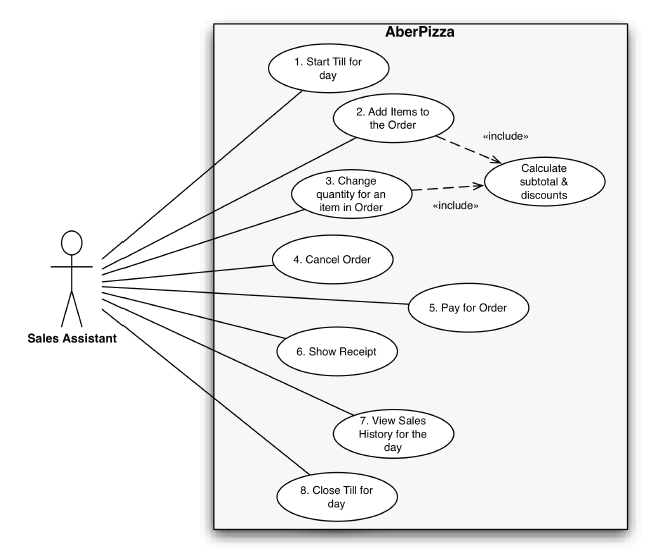
\includegraphics[width = 1\textwidth]{../Dia/use-case.PNG} 
	\caption{Use - Case diagram for the initial design}
	\label{fig5}
\end{figure}
Figure 5 shows the Use - Case diagram for the as it was supposed to be for finished application.\\
However I did not manage to implement all the there given features, but I wrote more about that in the Analysis part.\\
\newpage

\section{Analysis}

\textbf{How to run from Command Line}\\
You have to go to the directory where the .jar file is saved on your system.
If you are in the same Folder you can type the command java -jar AberPizza-stk4.jar\\

\textbf{Note:}
\begin{itemize}
\item Written in java 1.7 so an eclipse with version 1.6 might have problems with compiling it
\item Just works in the folder where it is placed(the one with "Menus" and "Tills" in it since it is depending on these 2 folder and I didn't managed to add them to the runnable jar file
\end{itemize}
\vspace{11pt}
In this assignment we was to create an piece of software that should be used in a local Pizza store called AberPizza.\\
The user should be able to choose from a couple of different Pizzas, available in 3 sizes:
Small, Medium and Large. There are also menus for sides and drinks. The user is able to add each item as often as they want and the program is to calculate the total price and where possible add 
discounts. There should also be a couple of "Admin" methods to get an over watch over all sales did an the current date and a couple of other methods. \\
However I was not able to implement all of this(because I started a bit late and had some struggles on the way). \\
In my program the user is able of adding any item from the different menus as often as they want. 
After the "checkout" the program calculates the total price for that order, and the till get saved as an .xml file.\\
My program don't has any of the admin methods, all my "Admin" menu can do is close the program.\\
The save method of my Till class saves the till as an xml file to order called "Tills".
As title of the tills it saves the date and time the order got saved, the format used for that is according to ISO standard 8601.\\
I also decided to save my Pizza, Sides and Drinks menus as an xml file which get loaded in DataManager. \\
I chose using an xml file as it makes it easier a lot easier to add and/or remove  Items to the menus as it would have been if I would have used hard coded menus. \\
I decided to but a bit more detailed description on how the classes work together on the Design part as I believe it is easier to understand that when one has the class diagrams on the same page. \\
So here I am going to write a short description of the most "important" classes in my design, more detailed information about the methods to all classes can be found in the JavaDoc.\\
\vspace{11pt}
\textbf{DataManager:}\\
Does all the data and method management between ItemPanel and OrderPanel.\\
Does fetch the information that goes on the till and than calls methods in Till and Order to calculate the Total for the order and saving.\\
Loads the menus for Pizza, Sides and Drinks from their xml files inside the "Menus" folder.\\   
\vspace{11pt}
\textbf{OrderPanel:}\\
Shows the list of items the customer wants to pay. It is this class where you set customer name for the current order and use the "Pay" button to "checkout" and save the current Till to an xml file. \\
\vspace{11pt}
\textbf{ItemPanel:}\\
Holds JButtons and JRadioButtons that are used to choose which menus the user wants to choose from. After the user did chose which one he wants to look at the menu is written to a JList.\\Sends the choosen item to DataManager which than uses intern and extern class methods to add it that item to the List in OrderPanel and to the current Order.\\
The standard start-up menu is the Large Pizza Menu. \\
\vspace{11pt}
\textbf{MainFrame:}\\
As the name suggest it creates the frame of for this program.\\
Than adds the ItemPanel(left side) and OrderPanel(right side) to it. It also creates an instance of DataManager and calls methods in ItemPanel, OrderPanel and DataManager to set up relationships between them and loading the standard start-up menu in ItemPanel.\\
\vspace{11pt}
\textbf{About the changes I made + self evaluation:}\\
I chose to make the changes to the given class diagram and create it the way I did as it seemed  to be the most reasonable for me. But I learn a lot about Object Oriented programming during this assignment and I now see ways of creating the design that would probably have been better/easier.\\
So I would ,if I were to design this program again, probably don't do it the same way even though the "core" of how I created it would probably be kind of the same. \\
I also "learnt" how to use Dia for drawing the diagrams, and learn more about LaTex.\\
An other important point I learn was to start as early as possible with an assignment in order to prevent myself from a very stressful time right before the deadline. 
\vline(11pt);
\textbf{Improvements}\\
If I would have more time, or wouldn't had started that late, my main goals for improving my program at the current state would be:
\begin{itemize}
\item Implementing of all requested features(loading till, discounts, showing of receipt,start and end till for day)
\item Improving of my GUI as it is not the best and prettiest one
\item Adding methods for "Admin" to add and/or remove new Pizza, Sides, Drinks to the program using nothing but the GUI
\end{itemize}
\vspace{11pt}

\section{JUnit}
In this section I am going to talk about the JUnit tests I wrote.\\
I wrote JUnit tests for all methods inside the .data package.\\
As they can be found inside the JavaDoc I am not going to write about all methods here, but write in general about what the test classes are doing.\\
\textbf{OrderTest:}\\
Here I tested the methods inside the Order class, and can say that all work fine, besides the methods that aren't implemented yet: getDiscount and getReceipt\\
\vspace{11pt}
\textbf{SuperItemTest:}\\
In here I tested all set and get methods for Pizza, Sides and Drinks classes as it 
is pretty important that all of them work perfectly.\\
\vspace{11pt}
\textbf{TillTest:}\\
Tests all methods inside the Till class, only problem here is the testsaveAndLoad method as I can't figure out on how to write that method probably\\
\vspace{11pt}
\textbf{OrderItemText}
In here did I test all methods of the OrderItem class\\
\vspace{11pt}
\textbf{CreatingMenus:}\\
Not really a test class as it test noting, but is JUnit code so I mention it here.\\
I uses this to generate the Menus for the program, by creating an ArrayList of Pizzas a separate one for Sides and another one for Drinks and than add the Pizza, Sides and Drinks to them using the methods I wrote.\\
I than save them using a save method similar to the one I used in Till and save the xml files to a folder called "Menus".\\
I mentioned earlier did chose to save the Menus as xml files as it makes it so much easier to remove and add items to the Menus which needing to actually hard-code anything into the program.\\
Just add a few lines of xml and the problem is solved.\\
\pagebreak
\section{Table of Testing}


\begin{longtable}{|p{2.5cm}|p{2.5cm}|p{2.5cm}|r|}
\hline
Requirements/Test & ActionPerformed & Pass/Fail & \multicolumn{1}{l|}{ScreenShots} \\ \hline
program loads start-up menu at start & loads start-up menu at start & pass & 1 \\ \hline
selecting the "Medium" radiobutton & changes the shown Menu to Medium Sized Pizza & pass & 2 \\ \hline
selecting the "Small" radiobutton  & changes the shown Menu to Small Sized Pizza & pass & 3 \\ \hline
clicking the "Drinks" Button & Showing the Drinks Menu & pass & 4 \\ \hline
Clicking the "Sides" Button & Showing the Sides Menu & pass & 5 \\ \hline
Clicking the "Pizza" Button & Shows the Pizza Menu according to the chosen radiobutton & pass & 6 \\ \hline
Selecting Item on the Menu by clicking on it & works & pass & 7 \\ \hline
pressing "Add" button after selecting an Item & adds the selected Item to the order List and Order & pass & 8 \\ \hline
Adding the previous item again & higher s the quantity at the order List by 1 - same for the Order & pass & 9 \\ \hline
Adding different Items & adds the new Items to the end of the order List & pass & 10 \\ \hline
Checks if name is set before you click "Pay" button & if name is not set it sends a warning & pass & 11 \\ \hline
creating a new till using the Menu & deletes the current order and order list and resets everything to Standard start-up & pass & no screen-shot \\ \hline
closing program from "admin" menu & works & pass & no screen-shot \\ \hline
checks if a item form the menu is chosen before you click "add" & if nothing is selected returns a warning & pass & 12 \\ \hline
saves till as xml file & works & pass & 13 \\ \hline
resets everything to standard start-up after check out & it wroks & pass & 14 \\ \hline
start till for day & not implemented  & fail & \multicolumn{1}{l|}{} \\ \hline
calculated subtotal & works but print out to the gui is not implemented & pass & no screen-shot \\ \hline
discounts & not implemented & fail & \multicolumn{1}{l|}{} \\ \hline
cancel order & can be done using "File" menu & pass & no screen-shot \\ \hline
pay for order & not implemented & fail & \multicolumn{1}{l|}{} \\ \hline
show receipt & not implemented & fail & \multicolumn{1}{l|}{} \\ \hline
view sales history of the day & not implemented & fail & \multicolumn{1}{l|}{} \\ \hline
close till for the day & not implemented & fail & \multicolumn{1}{l|}{} \\ \hline
checks of order list is empty & if empty it sends warning and prevents check-out & pass & 15 \\ \hline
\end{longtable}
\vspace{11pt}
\section{Other information}
All diagrams are drawn using Dia\\
JavaDoc is located in the Doc folder\\
LaTex files can be found in the LaTex Folder\\
Screen-Shots in the Screenshots folder\\
The tills that can be found inside the Till folder are a few test-Tills I have created\\
The initial design diagram(figure 1) and the use-case diagram (figure 5) are taking from the Assignment.

\newpage
\section{Screen - Shots}
 \begin{figure}[ht]
	\centering
 	\includegraphics[scale=0.4]{../Sceenshots/Capture.PNG} 
	\caption{Screen-Shot 1}
\end{figure}

 \begin{figure}[ht]
	\centering
 	\includegraphics[scale = 0.4]{../Sceenshots/Capture1.PNG} 
	\caption{Screen-Shot 2}
\end{figure}

\begin{figure}[ht]
	\centering
 	\includegraphics[scale = 0.4]{../Sceenshots/Capture2.PNG} 
	\caption{Screen-Shot 3}
\end{figure}

\begin{figure}[ht]
	\centering
 	\includegraphics[scale = 0.4]{../Sceenshots/Capture3.PNG} 
	\caption{Screen-Shot 4}
\end{figure}

\begin{figure}[ht]
	\centering
 	\includegraphics[scale = 0.4]{../Sceenshots/Capture4.PNG} 
	\caption{Screen-Shot 5}
\end{figure}

\begin{figure}[ht]
	\centering
 	\includegraphics[scale = 0.4]{../Sceenshots/Capture5.PNG} 
	\caption{Screen-Shot 6}
\end{figure}

\begin{figure}[ht]
	\centering
 	\includegraphics[scale = 0.4]{../Sceenshots/Capture6.PNG} 
	\caption{Screen-Shot 7}
\end{figure}

\begin{figure}[ht]
	\centering
 	\includegraphics[scale = 0.4]{../Sceenshots/Capture7.PNG} 
	\caption{Screen-Shot 8}
\end{figure}

\begin{figure}[ht]
	\centering
 	\includegraphics[scale = 0.4]{../Sceenshots/Capture8.PNG} 
	\caption{Screen-Shot 9}
\end{figure}

\begin{figure}[ht]
	\centering
 	\includegraphics[scale = 0.4]{../Sceenshots/Capture9.PNG} 
	\caption{Screen-Shot 10}
\end{figure}

\begin{figure}[ht]
	\centering
 	\includegraphics[scale = 0.4]{../Sceenshots/Capture10.PNG} 
	\caption{Screen-Shot 11}
\end{figure}


\begin{figure}[ht]
	\centering
 	\includegraphics[scale = 0.4]{../Sceenshots/Capture12.PNG} 
	\caption{Screen-Shot 12}
\end{figure}

\begin{figure}[ht]
	\centering
 	\includegraphics[scale=0.4]{../Sceenshots/xmlSave.PNG} 
	\caption{Screen-Shot 13}
\end{figure}

\begin{figure}[ht]
	\centering
 	\includegraphics[scale=0.4]{../Sceenshots/Capture.PNG} 
	\caption{Screen-Shot 14}
\end{figure}

\begin{figure}[ht]
	\centering
 	\includegraphics[scale = 0.4]{../Sceenshots/noCheckout.PNG} 
	\caption{Screen-Shot 15}
\end{figure}


\end{flushleft}
\end{document}